\chapter{Classification}
Classification is a form of supervised machine learning (in contrary to Clustering, see chapter \ref{chap:clustering}. It takes examples which we have identified whith classes and tries to learn a model that will predict the class of unknown examples. An example of use is to classify tumors as benign or malignant. We feed the classifier the features, such as size and shape, of known results. After the learning phase we can then use this classifier to predict if a given tumor is benign or not.

\section{K Nearest Neighbors}
K nearest neighbors is a simple but effective classification algorithm. The algorithm works by finding the k neirest neighbors of a given data point and chosing a class based on the labels of these k nearest neighbors. Basically using the majority vote of these neighbors to choose the data point's class. It is also possible to assign weight to the vote of the neighbors based on their distance.
\\
A known pitfall for the K Nearest Neighbor algorithm is that it needs to compare the data in question to all of the points from the dataset before we can know what the closest three points are. Therefor accuracy is easy to accomplish, but being fast is hard. Another way is to compare your data only to data within a certain radius. Other pitfalls include: problems with outliers and bad data.
\\
The confidence of this algorithm can be measured in two ways:
\begin{itemize}
\item Correct versus incorrect
\item Check the average vote confidence
\end{itemize}

\subsection{Code examples}
Two code approaches have been made. The first approach uses the \emph{sklearn} kit, the approach can be found in appendix \ref{code:knn}. The second approach shows a more basic KNN which illustrates it's fundamentals. This code can help you understand the basic building blocks of the algorithm and let you see where it's pitfalls are. The code can be found in appendix \ref{code:mknn}.

\section{Support Vector Machines}
A SVM is a bineairy classifier. It tries to classify the examples by seperating them lineairly. This is done by maximising the distance between the seperating plane and the closest example of both classes, as shown in figure \ref{fig:svm}

\begin{figure}
\centering
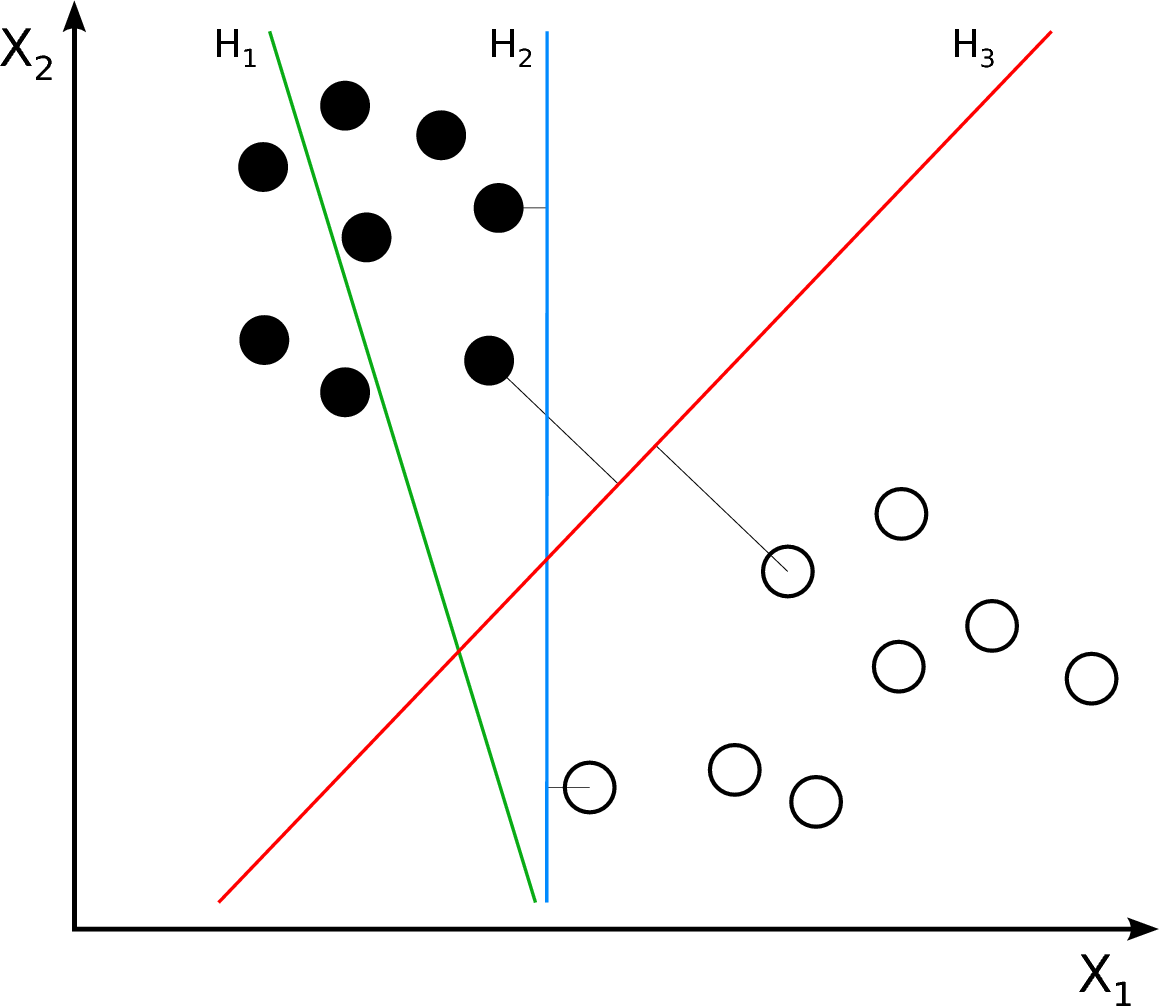
\includegraphics[width=0.4\textwidth]{images/svm.png}
\caption{\label{fig:svm} Shows three seperation planes, H1 is not a good seperating plane, H2 and H3 are acceptable.}
\end{figure}

\subsection{Support Vector Machine Regression}
It is possible to use SVMs to learn linear regression lines, as shown in our code example \ref{code:manualregression}, however we will not discuss in depth how this works.